\chapter{Convolutional Neural Network}

\section{Neurone convoluzionale}
\begin{wrapfigure}{l}{.6\linewidth}
	\vspace{-.2cm}
	\centering
	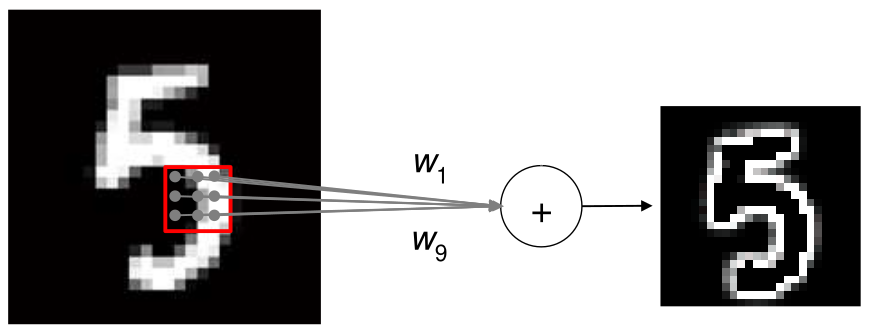
\includegraphics[width=.9\linewidth]{Picture/Convolutional_Neuron}
\end{wrapfigure}
È un neurone che applica un filtro all'immagine ed estrae la tessa feature da tutta l'immagine. Per fare questo opera come un normale neurone che calcola una combinazione lineare degli input, ma gli input avranno dei vincoli spaziali, in particolare saranno una matrice quadrata di pixel che con la convoluzione viene filtrata dai parametri del neurone. I parametri saranno appressi attraverso la backpropagation e non si dovranno più progettare a mano i filtri per estrarre le features.

Per fare in modo che dopo l'operazione di filtraggio il risultato abbia le stesse dimensioni dell'immagine originale si fa zero padding. 

Se stiamo trattando immagini colorate trattiamo ogni canale in modo indipendente, ad esempio se costruiamo dei filtri $3\times3$ ogni neurone apprenderà $27$ parametri, $9$ per ogni filtro. I risultati del filtraggio dei tre canali è poi sommato per generare la feature map.

\section{Complessità del layer convoluzionale}
Il numero di parametri che devono essere appresi per ogni livello convoluzionale sarà dato dal numero di feature map che vlgiamo ottenere $n_{out}$ (numero di filtri nel livello) per la dimensione del filtro + 1 per il numero di canali in ingresso; questi saranno 3 per le immagini a colori 1 per e immagini in scala di grigi e  il numero di feature map estratte al livello precedente se stiamo considerando un generico layer all'interno della rete.  In formule possiamo scrivere:
\begin{equation}
	N_{par} = n_{out} \cdot (1+F^2)\cdot n_{ch}
\end{equation}
Dove $F$ rappresenta il lato del filtro.
\subsection{Complessità della rete}
Ogni neurone convoluzionale restituisce come output un'immagine delle stesse dimensioni dell'immagine originale. Dopo che abbiamo estratto tutte le feature che ci interessano quindi dobbiamo tornare a una FCN per poter fare la classificazione. Per fare questo semplicemente serializziamo ogni feature map e la concateniamo con le altre.

Il collo di bottiglia diventa quindi il layer di passaggio tra CNN e FCN, dato che al posto di avere un neurone per ogni pixel dell'immagine originale avremo un neurone per ogni pixel di ogni feature map, e queste possono essere anche molte.

\subsection{Ridurre la complessità}
Per ridurre la complessità possiamo trattare le feature map come immagini e sottocampionarle. Per ridurre le dimensioni delle feature map abbiamo due alternative.

\subsubsection{MaxPolling}
\begin{wrapfigure}{r}{.5\linewidth}
	\vspace{-.5cm}
	\centering
	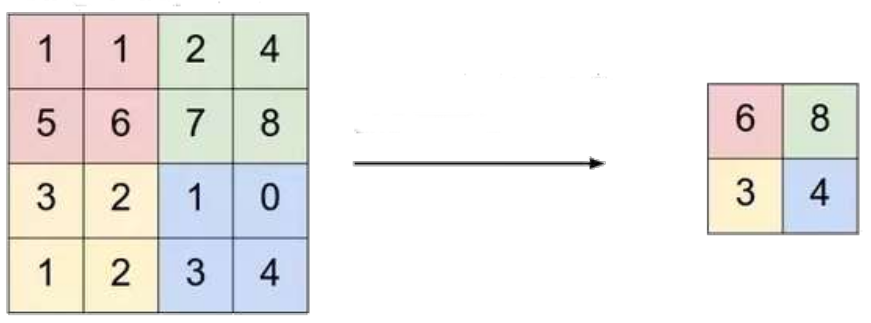
\includegraphics[width=.9\linewidth]{Picture/MaxPolling}
\end{wrapfigure}
Il MaxPolling consiste nel dividere l'immagine in celle da 4 pixel e per ogni cella prendere solo il valore maggiore. In questo modo dimezziamo la dimensione dell'immagine e dato che prendiamo solo il valore più grande e non facciamo la media eseguiamo anche un'operazione di \textbf{Non Maxima Suppression}, si è visto che questo aggiunge robustezza alle traslazioni.

\subsubsection{Convolve and Stride}
In questo caso ogni convoluzione ha un passo maggiore di 1, questo significa che il flitro non si sposta sull'immagine pixel per pixel ma fa dei salti.

Questa tecnica non prevede la Non Maxima Suppression, ma è parte integrante del processo di filtraggio e non deve essere aggiunta come layer intermedio tra 2 layer di neuroni. Questo rende la tecnica del convolve and stride più flessibile e di fatto ha soppiantato il MaxPolling nelle moderne architetture.

\section{LeNet5}
Presentiamo l'architettura della LeNet5 che prevede 2 livelli convoluzionali da 6 e 16 neuroni, intervallati da 2 livelli di MaxPolling, si passa poi 3 livelli FC. 
\begin{center}
	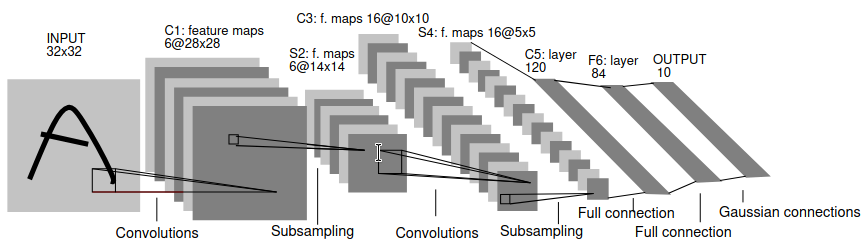
\includegraphics[width=.8\linewidth]{Picture/LeNet_5}
\end{center}
Il tasso d'errore della LeNet5 con l'architettura in figura è di $0.95\%$, questo miglioramento nelle performance è accompagnato anche da una riduzione della complessità della rete rispetto alla LeNet300, in particolare il numero di parametri necessari alla LeNet5 è meno di $\frac{1}{3}$ dei parametri necessari alla LeNet300.

\section{Receptive Field}
Il receptive field di una feature indica quanti pixel dell'immagine originale sono stati usati per generare la feature. Ad esempio un filtro $3\times3$ ha un receptive field di 9 pixel.

Nell'immagine si vede una rappresentazione 2D del receptive fiel della LeNet5. Notiamo che:

\begin{wrapfigure}[4]{r}{.5\linewidth}
	\vspace{-.5cm}
	\centering
	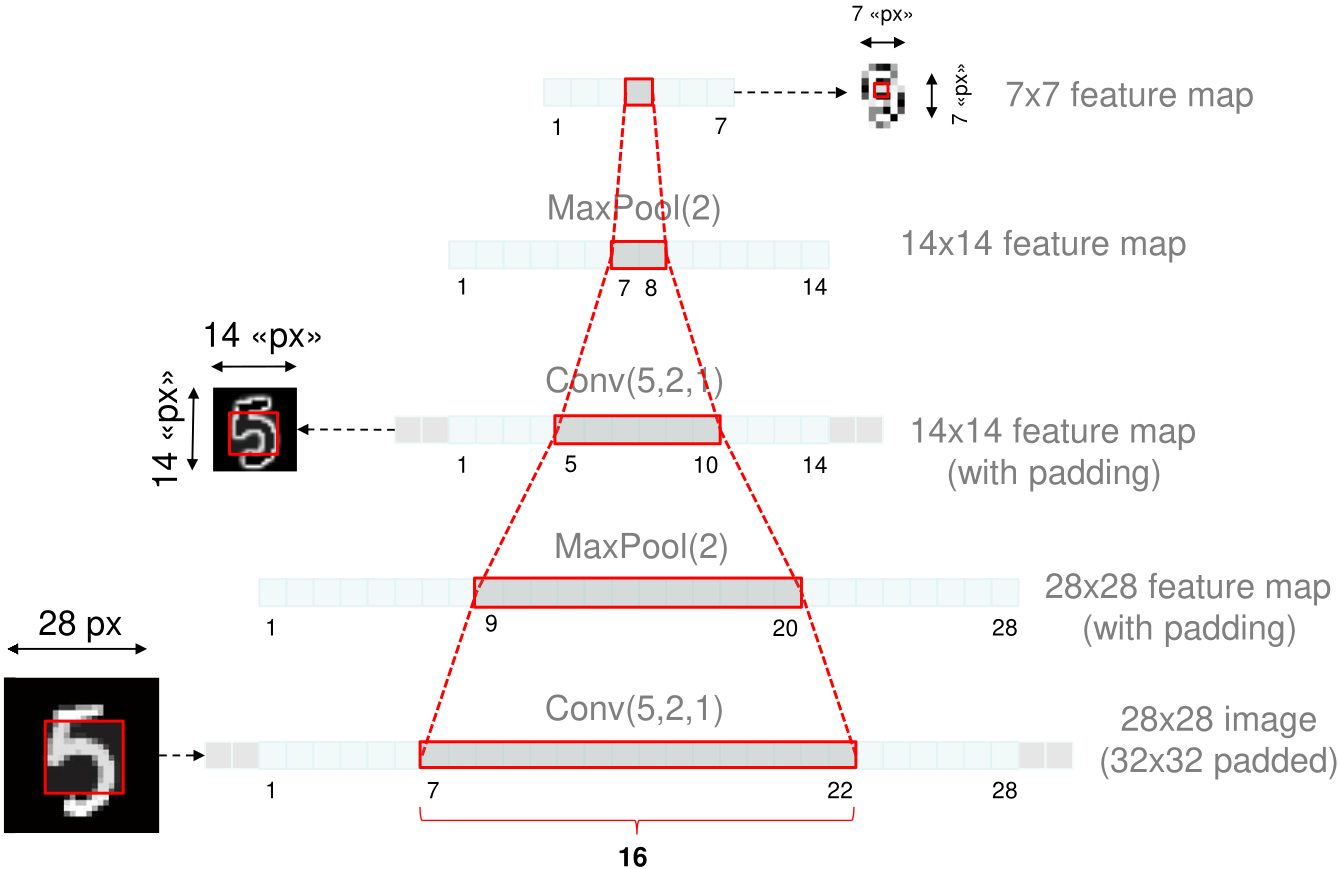
\includegraphics[width=\linewidth]{Picture/Receptive_Field}
\end{wrapfigure}
\ 
\vspace{-.5cm}
\begin{itemize}
	\item i livelli di MaxPolling sono quelli che più di tutti influiscono sul receptive fiel, raddoppiandolo;
	\item i filtri aumentano la dimensione del receptive field per effetto del padding.
\end{itemize}

	Che si usi il MaxPolling oppure il convolve and stride il subsampling dell'immagine consente di aumentare il receptive field. Questo è molto importante perché vogliamo che ogni feature (che al passando dall'ultimo livello convoluzionale al primo fully connected è costituita da un pixel) trasporti più informazione possibile.
	
\section{Da fully connetted a fully convolutional}
\subsection{Riconosimento del testo}
Ora che abbiamo progettato una rete in grado di raggiungere elevata acccuratezza nel riconoscimento dei singoli caratteri vorremmo poter leggere il testo scritto su in immagine. Per fare questo abbiamo bisogno di individuare i caratteri prima di riconoscerli. L'approccio naif consiste nel:
\begin{itemize}
	\item aggiungere una classe di backgound che non corrisponde a nessun carattere;
	\item aggiungere una classe che corrisponde all'intersezione di 2 caratteri, anche questa non corrisponde a nessun carattere;
	\item fare zigzag per l'immagine con passo di 1 pixel per individuare tutti i caratteri.
\end{itemize}
Questo approccio è molto inefficiente, dato che ogni pixel viene elaborato molte volte, tutte le elaborazioni sono indipendenti e la maggior parte di queste sono ridondanti o non portano informazione.
\subsection{Sliding Window}
Al posto che ritagliare l'immagine in quadrati della stessa dimensione delle immagini di training posso usare delle finestre di dimensione arbitraria, tanto i livelli convoluzionali si comportano come filtri e possono essere applicati a qualsiasi immagine.

\begin{wrapfigure}{l}{.53\linewidth}
	\vspace{-.25cm}
	\centering
	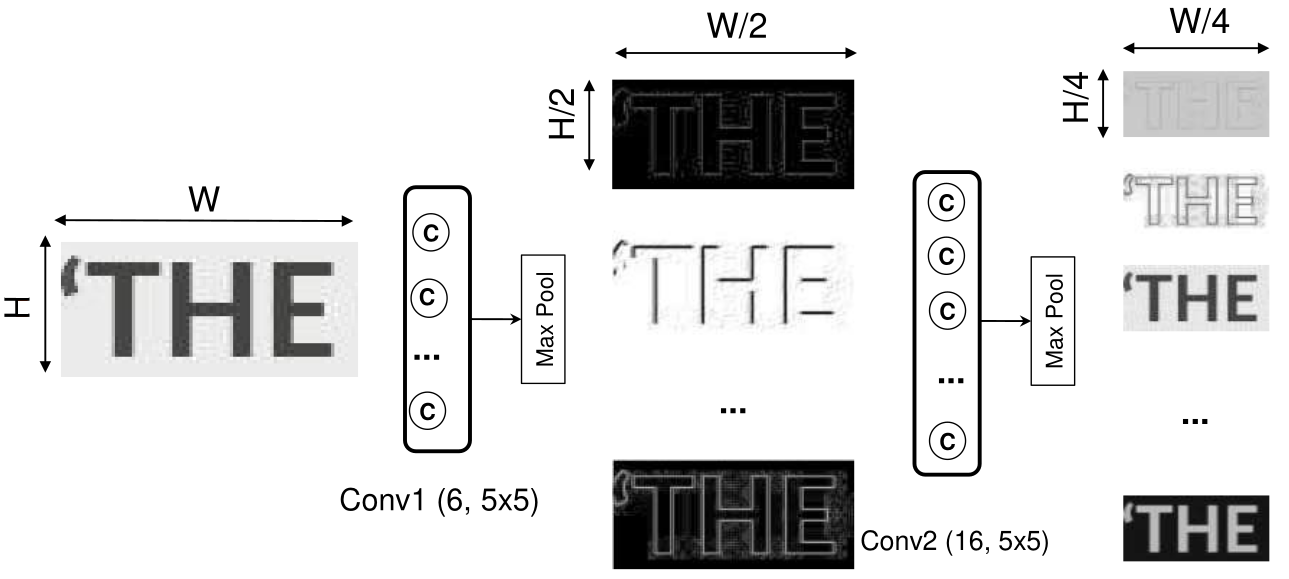
\includegraphics[width=\linewidth]{Picture/Sliding_Window_LeNet_5}
\end{wrapfigure}
Nella figura si vede l'effetto dei neuroni convoluzionali che permettono di estrarre le feature per le quali sono stati addestrati da un immagine qualsiasi. Si vede anche l'effetto del MaxPolling che dopo ogni livello dimezza la dimensione delle features. 

Rimane però un problema, dato che la rete termina con dei livelli fully connected questi hanno bisogno di un vettore di input di dimensione fissata e non possono adattarsi alle dimensioni della finestra arbitraria che abbiamo scelto.

\subsection{Equivalente convoluzionale}
\begin{wrapfigure}{r}{.5\linewidth}
	\vspace{-.25cm}
	\centering
	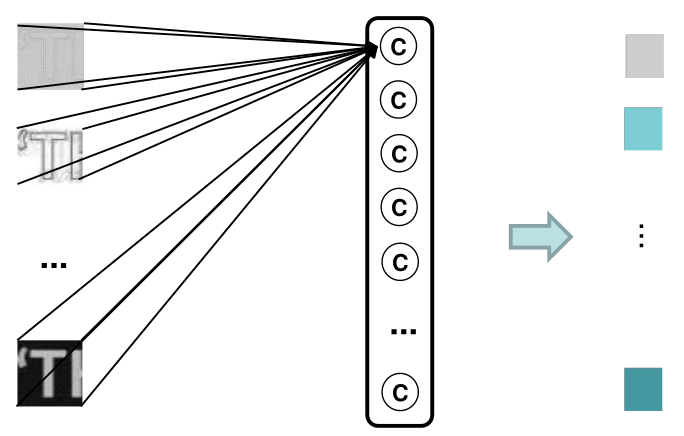
\includegraphics[width=\linewidth]{Picture/FC_To_CNN}
\end{wrapfigure}
Sostituiamo quindi i livelli fully connected con dei livelli convoluzionali. Consideriamo il primo livello FC, questo riceve in input un certo numero di features map (FM) di dimensione fissa. Per ogni FM avrà un peso per ogni pixel. Possiamo quindi trasformare questo neurone in un filtro semplicemente trattandolo come tale senza bisogno di cambiare i pesi. I neuroni convoluzionali ottenuti trasformando un layer FC sono detti \textbf{narrow}. Anche il livello di output può essere sostituito con un livello convoluzionale collegato poi alla funzione Soft-Max.

Una volta fatte queste sostituzioni siamo pronti per applicare la rete fully convolutional (CNN) all'intera immagine
\begin{center}
	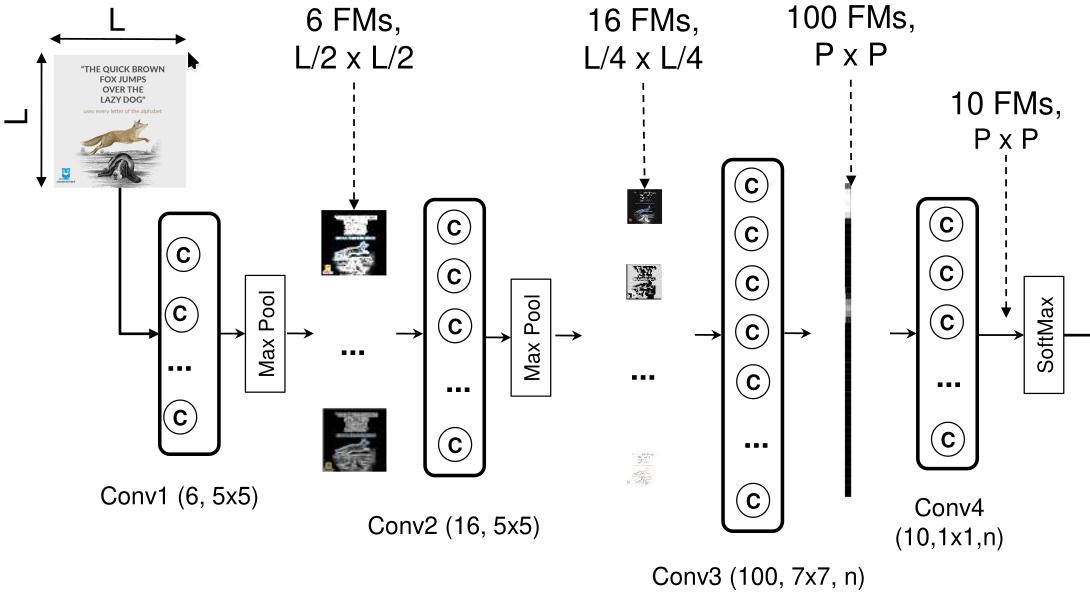
\includegraphics[width=.75\linewidth]{Picture/CNN}
\end{center}
Dove:
\begin{equation}
	P = 1 + \frac{L -(f_{dim} \cdot 2^{n_{pools}})}{4}
\end{equation}
e $f_{dim}$ è la dimensione del filtro narrow del primo livello FC tradotto (in questo caso la dimensione è 7), e $n_{pools}$ è lo stride (In questa rete quindi si combinano convolve and stride e MaxPolling).
\subsection{Interpretare i risultati}
{\Huge DA RISCRIVERE}

\begin{wrapfigure}{r}{.4\linewidth}
	\vspace{-.25cm}
	\centering
	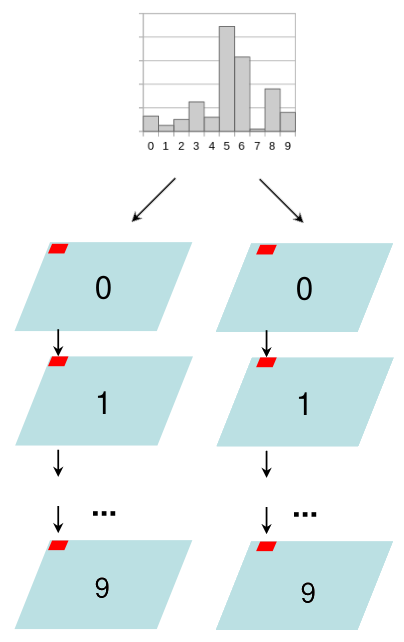
\includegraphics[width=\linewidth]{Picture/Post_CNN}
\end{wrapfigure}
Ora che abbiamo ottenuto delle feature map dobbiamo interpretarle. Per fare questo possiamo riutilizzare il classificatore FC che avevamo prima convertito in convoluzionale e passare a questo dei vettori di lunghezza 10, ciascun vettore conterrà il pixel $i,j$ di ciascuna delle 10 FM che abbiamo estratto con la rete CNN. Ogni vettore può quindi essere classificato e fornirci in output un carattere. Nel caso della LeNet5 si ottengono 10 FM $19\times19$, saremo quindi in grado di riconoscere al massimo $19\times19 = 361$ caratteri.

 Il risultato di questa prima interpretazione potrebbe essere ancora poco soddisfacente, potrebbero infatti esserci dei doppioni e delle lettere sbagliate. A valle di questo passaggio quindi si usano dei language model e altre reti per raffinare il risultato da un punto di vista semantico. 
 